% TeX encoding = utf8
% TeX spellcheck = pl_PL 
\documentclass[a4paper, 12pt]{article}
\usepackage[utf8]{inputenc}
\usepackage[polish]{babel}
\usepackage{polski}
\usepackage{graphicx}
\usepackage{listings}
\usepackage{amsfonts}
\usepackage{geometry}
\usepackage{multicol}


\newgeometry{tmargin=3cm, bmargin=3cm, lmargin=2cm, rmargin=2cm}

\pagestyle{empty}

\begin{document}
	
\section{Abstrakt}
Celem projektu jest budowa zespołu robotów mobilnych o zmiennym trybie lokomocji, jako patformy do impementacji algorytmów grupowej współpracy robotów oraz robotycznych gier zespołowych.


\section{Elementy}
\subsection{Robot mobilny o zmiennym trybie lokomocji}
Najważniejszym komponentem projektu jest mobilna platforma robotyczna o zmiennej lokomocji.Bazuje ona na dwukołowym robocie balansującym, który może poruszać się w pozycji pionowej(balansującej) oraz w poziomej z dodatkowym punktem podparcia. Zastosowanie tego typu platformy stwarza wiele możliwości wykorzystania oraz upraszcza konstrukcję robota. Wymiary nie przekraczają 18x8 cm w podstawie oraz 20 cm wysokości. Podstawowym trybem poruszania się platformy jest pozycja pozioma, do której utrzymanania niezbędne są czujniki inercyjne oraz odpowiedni sterownik. Dodatkowo na platformie zostaną zainstalowane czujniki stanu otoczenia takie jak dalmierze, czujniki podłoża oraz opcjonalnie kamera w celu umożliwienia realizacji algorytmów wizyjnych. Projekt w początkowej fazie zakłada konstrukcję kilku takich samych robotów, których grono można dowolnie powiększać. 

\subsection{System lokalizacji}
Ważnym elementem realizacji algorytmów sterowania grupą robotów jest ich lokalizacja w przestrzeni. Do realizacji tego zadania zostanie użyta metoda trilateracji. Realizację tego zadania umożliwi zastosowanie specjalistycznego transceivera radiowego działąjącego w technologii UWB, który zapewnia możliwość pomiaru odległości pomiędzy nadajnikiem a odbiornikiem z dokłądnością do 10 cm. Rozmieszczenie nadajików w zamikniętej przestrzeni oraz odbiornika na każdym z robotów umożliwi lokalizację kazdego z robotów na przestrzeni do 200 m2, zakłądając lokalizację 2D oraz do 200 m3 gdy lokalizacja odbywała się będzie w 3 wymiarach. Dodatkowo w celu poprawy dokładności do wyznaczania położenia zostaną wykorzystane odczyty z czujników inercyjnych na każdym robocie oraz kąty obrotu kół robota. Fuzja tych 3 elementów powinna zapewnić wystarczającą dokłądność zarówno przy przeyzyjnych opracajach jak i podczas szybkiego poruszania się w przestrzeni.

\begin{figure}
\centering
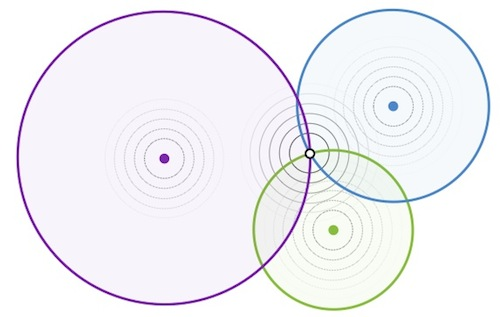
\includegraphics[width=10cm]{img/lokalizacja.jpg}
\caption{Wyznaczanie położenia}
\label{fig:lokalizaja}
\end{figure}


\subsection{Komunikacja}
Klejnym elementem niezbędnym podczas zespołowej pracy robotów jest ich wzajemna komunikacja. Do tego celu zostanie użyta bezprzewodowa sieć LAN w standardzie 802.11n. Na każdym robocie zostanie zainstalowany moduł WLAN który będzie łączył się do centralnego punktu dostępu. Takie połączenie umożliwi szybką i prostą w użyciu komunikację zmiennej liczby elementów. Dodatkowo standard zapewnia odpiwiednią stabilność oraz kontrolę poprawności przesyłanych danych. 

\subsection{Sterowanie}
Sterowanie systemem będzie odbywało się przez dostęp sieciowy z poziomu dedykowanej aplikacji. Użytkownik będzie miał możliwość odczytu stanu poszczególnych robotów oraz wysyłania do nich komend sterujących. Wykonanie algorytmu sterowania będzie odbywało się w sposób rozproszony tj. każdy robot będzie znał stan wsztstkich robotów w systemie i bedzie mógł wpływać na stan pozostałych w zależności od priorytetu zdażenia. Dodatkowo istnieje możlwość implementacji nadrzędnego algorytmu syerującego, wykonywanego z poziomu aplikacji sterującej na urządzeniu podłązonym do sieci systemu. Kolejnym aspeketm jest możliwość autonomicznego działania poszczególnych robotów oraz możliwość sterowania bezpośedniego przy pomocy dowolnego urządzenia posiadającego przeglądarkę internetową i podłączonego do sieci. 

\subsection{Platforma sprzętowa}
Istotną rzecą z punktu widzenia działania systemu jest platforma sprzętowa na której uruchomione zostanie oprogramowanie sterujące. Projekt zakłada użycie systemu czasu rzeczywistego do kontroli nad procesami priorytetowymi takimi jak kontrola silników, odczyty danych z czujników krytycznych, utrzymanie robota w odpowiednej pozycji, określanie lokalizacji. Do tego celu zostanie wykorzystana platforma prototypowa STM32 nucleo, zawierająca w sobie 32-bitowy mikrokontroler z rdzeniem ARM, niezbędne do działania komponenty pasywne oraz zintegrowwany programator i debugger. Poza systemem czasu rzeczywistego, w celu zapewnienia możliwiej jak najszerszej funkcjonalności, zostanie użyty system czasowo niedeterministyczny, odpowiedzialny za wymianę informacji na wyższym poziomie abstrakcji, wysyłaie komend do mikrokontrolera sterującego oraz realizację zadań złożonych obliczeniowo lub wymagających większych zasobów sprzętowych. Do tego celu zostanie wykorzystana jedna z platform z rodziny Raspberry Pi z systemem opartym o jądro LINUX. Na tym poziomie możliwa będzie interpretacja języków skryptowych, które zapewniają szybką implementację i przenośność. Dodatkowo z poziomu platformy Raspberry możliwe będzie zaprogramowanie mikrokontrolera sterującego bez potrzeby fizycznego podłączania robota do komputera typu PC. Zapewnia to przede wszystkim możliwość szybkiego programowania wielu robotów w tym samym czasie. 

\section{Funkcjonalność}
Projekt ma nieograniczone możliwości zastosowań, dlatego może służyć jako baza do bydowy algorytmów i zadań dla grupy robotów. Jednym z głównych zastosowań jest możliwość transportu obiektów w określone miejsce w przestrzeni. Roboty mogą wspólnie przesuwać obiekty i pomagać sobie gdy jeden robot nie jest w stanie przemieścić obiektu. Pozwala to tworzyć proste gry polegające na opracowaniu najoptymalniejszego algorytmu przemieszczania obiektów. 

\begin{figure}
\centering
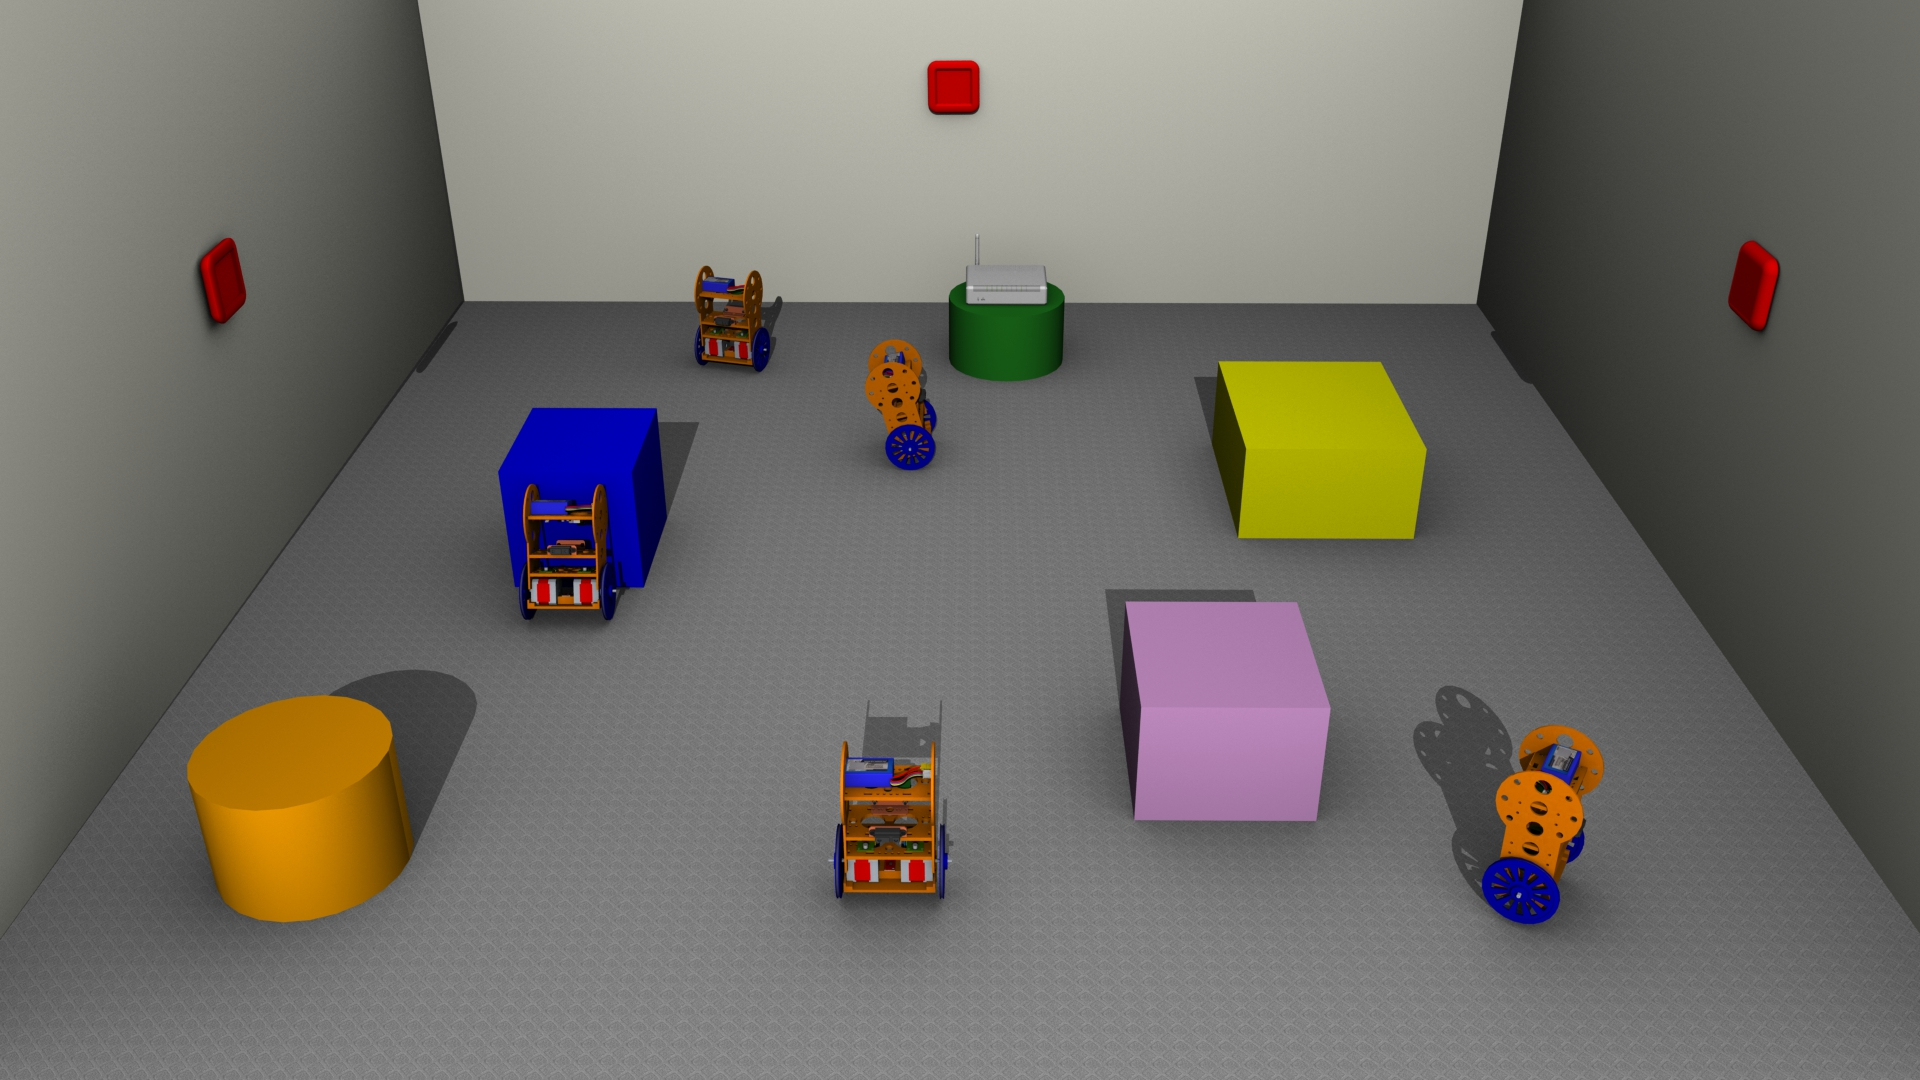
\includegraphics[width=15cm]{img/grupa.jpg}
\caption{Przykładowy senariusz użycia}
\label{fig:grupa}
\end{figure}

\section{Obecny stan wiedzy}
Grupy robotów to szybko rozwijająca się dziedzina stwarzająca ogromne możliwości. W życiu codziennym mamy doczynienia coraz częściej ze współbieżynmi systemami. Wymiana informacji pomiędzy poszczególnymi elementami systemu pozwala na efektywniejszą i szybszą pracę. Dużo słyszy się o nowoczesnych technologiach Internetu rzeczy, staje się to coraz bardziej naszą codziennością. Dlatego też projekt grupy robotów stara się wykorzystywać technilogie które wchodzą w jego skład. Jest to dobra okazja do przysfojania i zgłębiania elementów rozproszonych sposobów rozwiązywania problemów i współpracy. Co więcej rozwiązanie to tworzy coś w rodzaju internetu robotów, co jest wysoce innowacyjne. 

\section{Postęp Pracy}
Obecnie trwają prace nad pierwszym prototypem robota bedącego podstawowym elementem systemu. Do wykonania posostało jeszcze wiele pracy projektowej oraz implementacyjnej. Chcielibyśmy aby projekt stał się narzędziem dla studentów, dlatego przykładamy dużo uwagi do dobrej dokumentacji projektu oraz prostoty użytkowania. Aby zapewnić odpowiedni poziom niezawodności i mozliwość długotrwałej pracy systemu, jesteśmy zmuszeni do używania wysokiej jakości komponentów, oraz tworzenia własnych rozwiązań z zakresu elektroniki i elementów mechanicznych. Warto podkreslić że nad projektem pracuje grupa osób wo której każdy odpowiedzialny jest za swoją częśc projektową. Jak w każdym projekcie do wykonania potrzebne są pewne zasoby finansowe. W naszym przypadku kolejnym etapem powinien być zakup cześci, które umożliwią budowę kilku robotów i rozpoczęcia testów nad algorytmami grupowymi. 

\begin{figure}
\centering
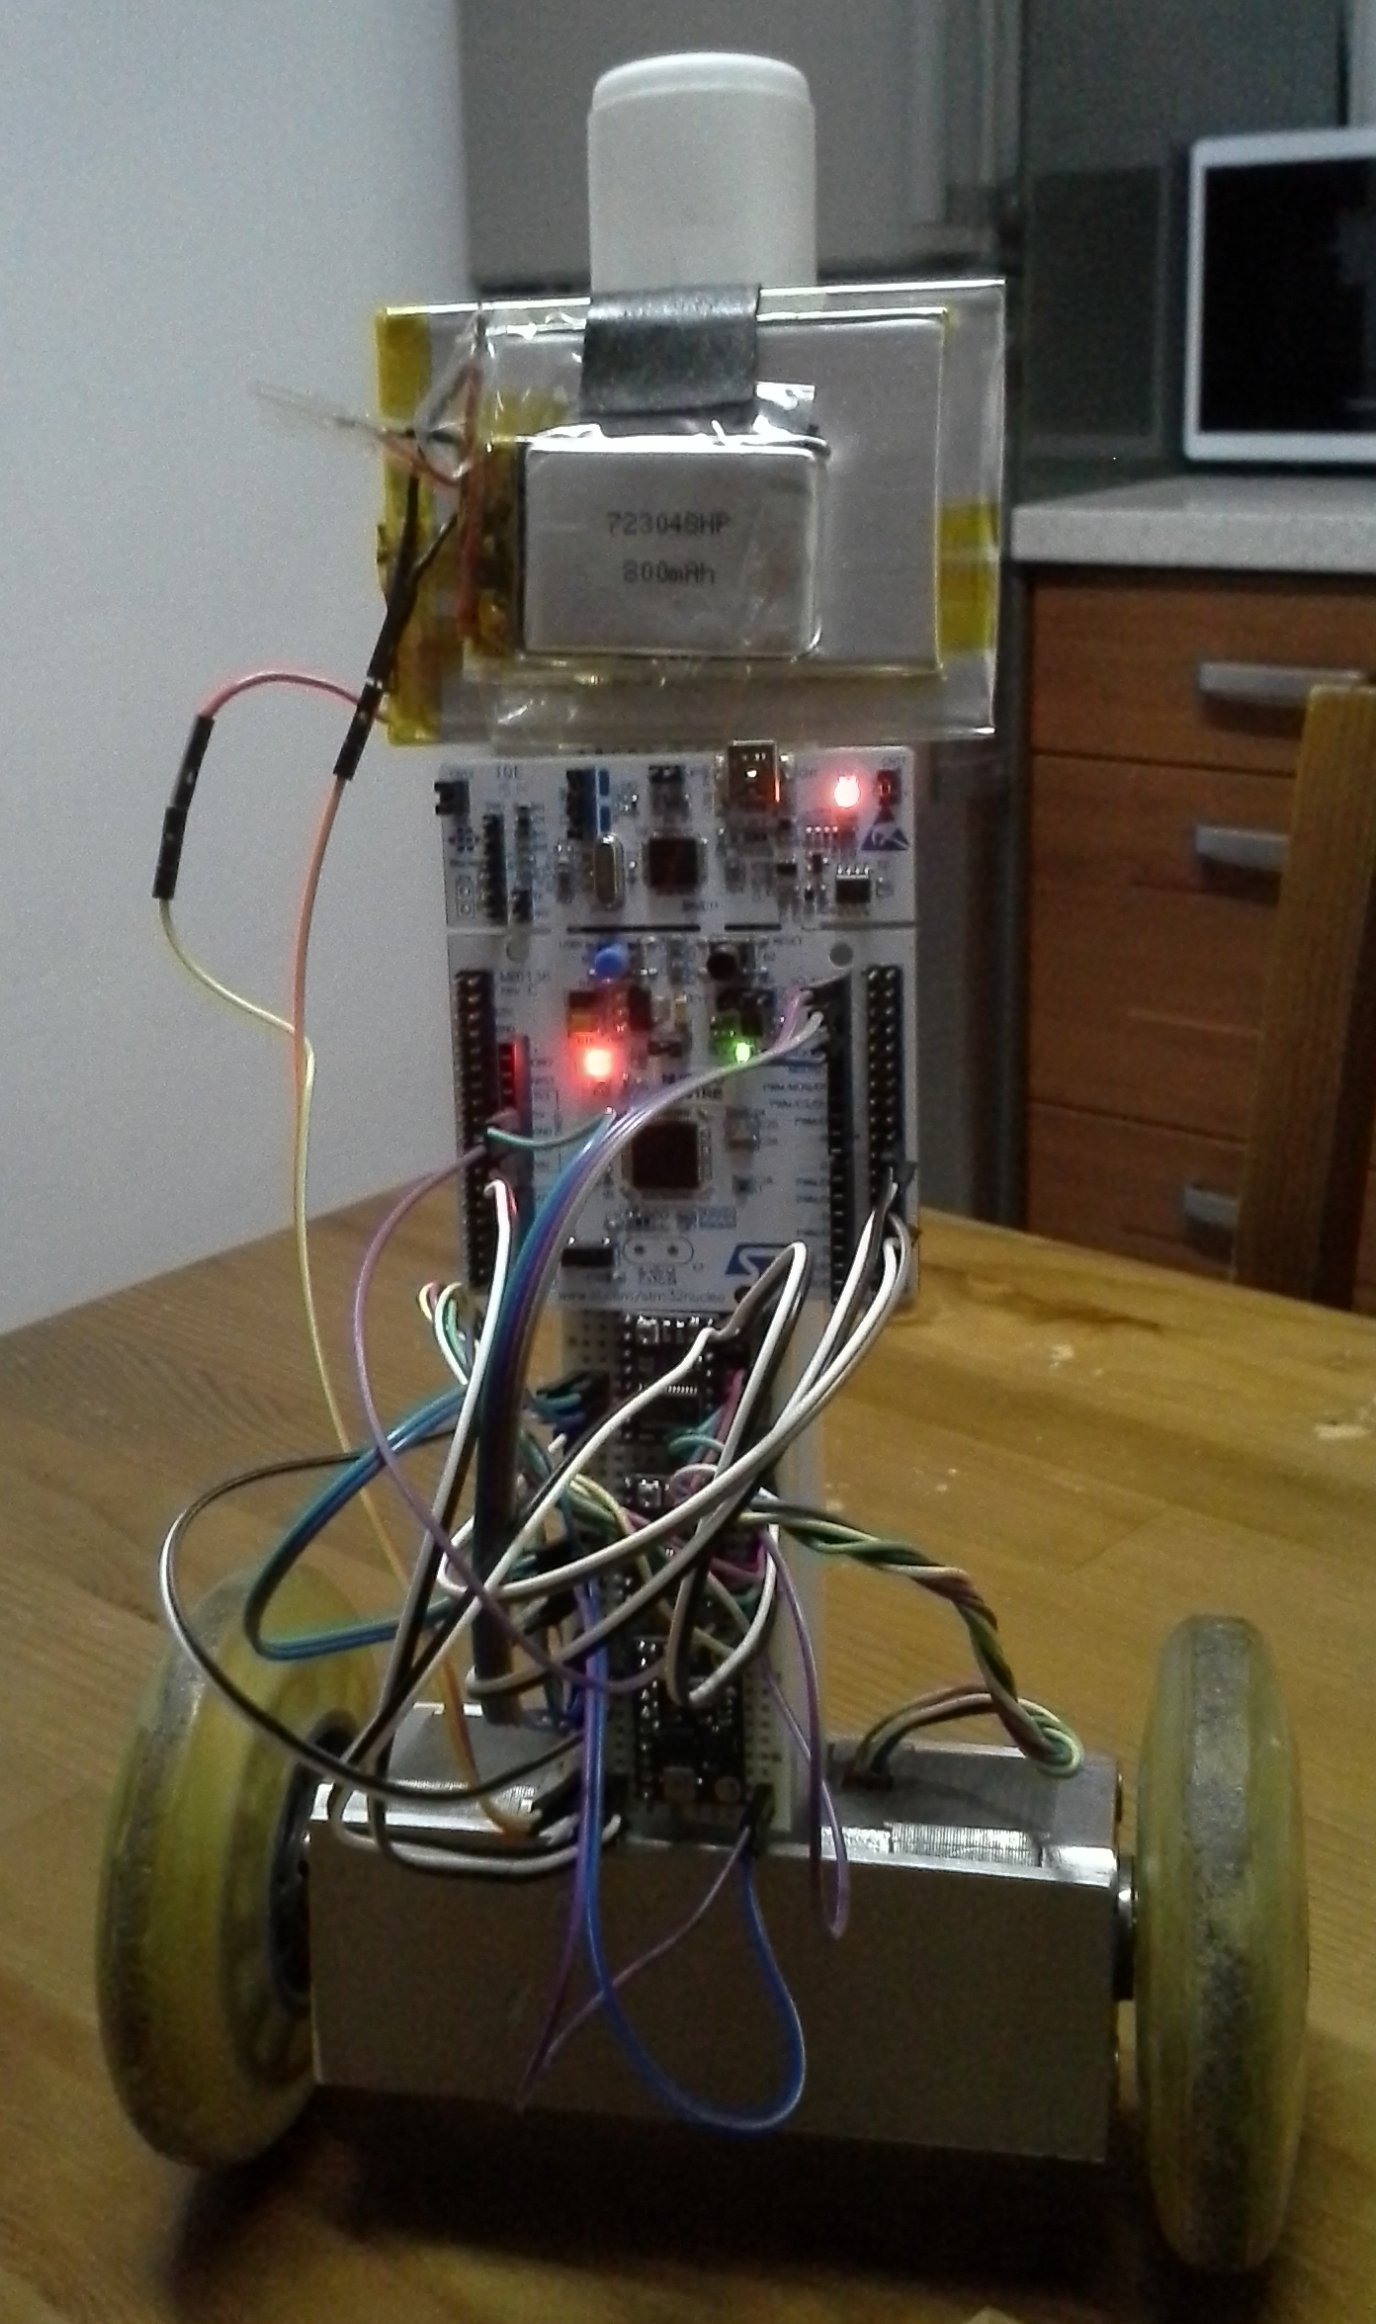
\includegraphics[width=5cm]{img/prototyp.jpg}
\caption{Pierwszy prototyp}
\label{fig:prototyp}
\end{figure}

\section{Wykonanie}
Elementy mechaniczne platformy robotycznej będą wykonane technologią druku 3D. Są to: mocowania silników, szkielet robota, uchwyty do komponentów elektronicznych oraz koła. Na płycie głównej robota będą znajdowały się: mikrokontroler sterujący wraz z programatorem, sterowniki silników, transceiver radiowy, moduł WiFi, moduł zasilający oraz gniazda czujniki i baterię. IMU będzie zamocowane w punkcie na osi obrotu kól aby umożliwić prezyzyjny pomiar kąta wychylenia. Czyjniki takie jak dalmierze zostaną umieszczone na korpusue robota. Istotnym elementem konstrukcji jest zderzak który będzie miał kontakt z podłożem oraz elemtami fizycznymi. Zostanie on wykonany z elastycznego tworzywa aby zapewnić odpowiednią amortyzację.

\begin{figure}
\centering
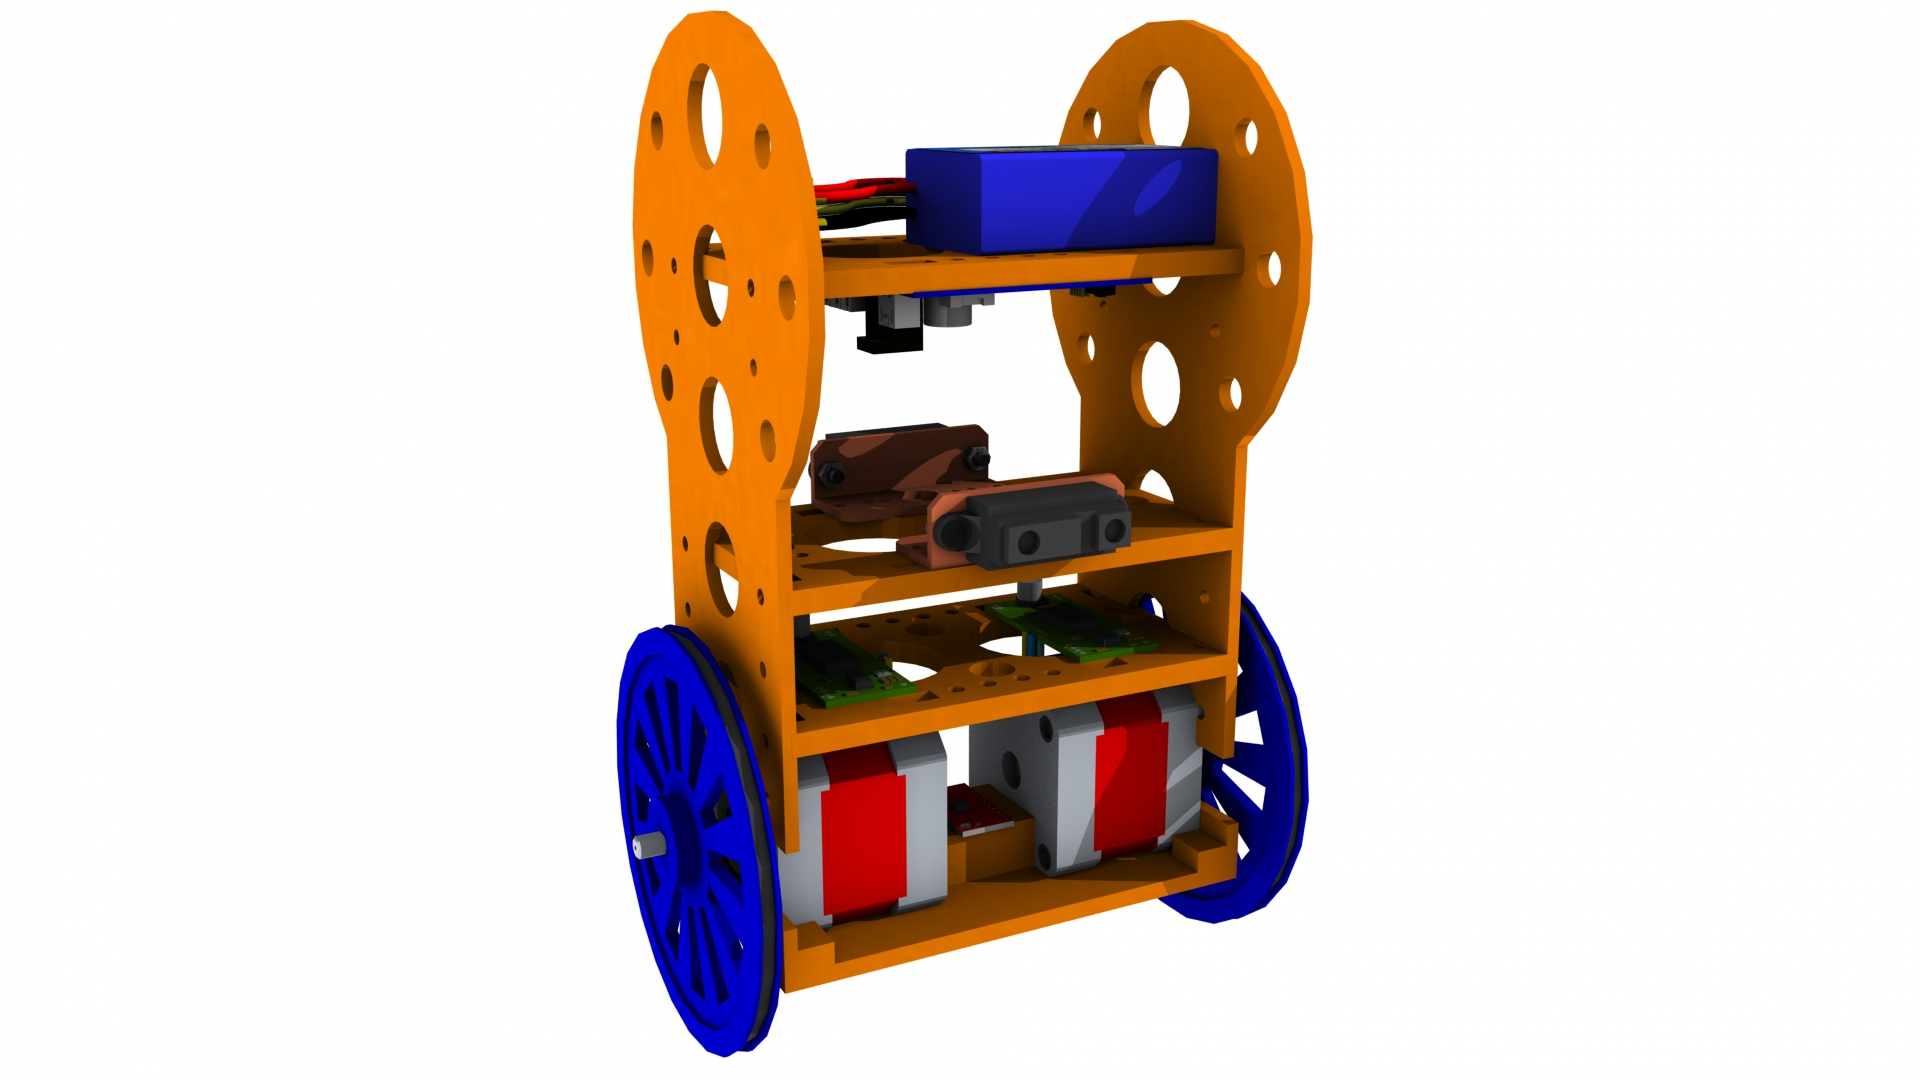
\includegraphics[width=14cm]{img/mrys.jpg}
\caption{Projekt robota}
\label{fig:projekt}
\end{figure}

\section{Komponenty}
\begin{table}[ht]
	\normalsize
	\begin{tabular}{ll}

    Silnki krokowe typu NEMA 17\\
    Sterowniki DRV8825\\
    STM32 nucleo board\\
    ARM v7< board\\
    Transceiver DMW1000 (lokalizacja)\\
    Moduł WiFi (komunikacja z siecią)\\
    Diody WS2812B (sygnalizacja aktualnego stanu robota)\\
    Czujniki odległości SHARP (cyfrowe)\\
    IMU MPU6050\\
    Gniazda do podłączenia innych czujników (w zależonści od wykorzystania)\\
    
	\end{tabular}
\end{table}


	
\end{document}


